\documentclass[12pt]{article}
\usepackage[utf8]{inputenc}
\usepackage[T1]{fontenc}
\usepackage{amsmath}
\usepackage{amsfonts}
\usepackage{amssymb}
\usepackage[version=4]{mhchem}
\usepackage{stmaryrd}
\usepackage{bbold}
\usepackage{graphicx}
\usepackage[export]{adjustbox}
\graphicspath{ {./images/} }

\usepackage{listings} % Required for insertion of code
\usepackage{xcolor} % Required for custom colors

% Define custom colors
\definecolor{codegreen}{rgb}{0,0.6,0}
\definecolor{codegray}{rgb}{0.5,0.5,0.5}
\definecolor{codepurple}{rgb}{0.58,0,0.82}
\definecolor{backcolour}{rgb}{0.95,0.95,0.92}

% Setup the style for code listings
\lstdefinestyle{mystyle}{
    backgroundcolor=\color{backcolour},   
    commentstyle=\color{codegreen},
    keywordstyle=\color{magenta},
    numberstyle=\tiny\color{codegray},
    stringstyle=\color{codepurple},
    basicstyle=\ttfamily\footnotesize,
    breakatwhitespace=false,         
    breaklines=true,                 
    captionpos=b,                    
    keepspaces=true,                 
    numbers=left,                    
    numbersep=5pt,                  
    showspaces=false,                
    showstringspaces=false,
    showtabs=false,                  
    tabsize=2
}

% Activate the style
\lstset{style=mystyle}

\title{Assignment 2: Entanglement entropy and compression of quantum states }


\author{Instructor: Lesik Motrunich\\
TA: Liam O'Brien}
\date{}


\begin{document}
\maketitle
Ph 121C: Computational Physics Lab, Spring 2024

California Institute of Technology

Due: 4pm Tuesday, April 30, 2024









\section*{5 Assignment: entanglement entropy and state compression}



\subsection*{5.3 Truncation error of Schmidt decomposition}
Consider again the Ising ground state at representative values of the control parameter $h / J$, using open boundary conditions. Perform the Schmidt decomposition at the middle of the chain and compute the approximate ground state arising from truncating the factorization at $k$ ranging from 1 to $2^{L / 2}$. For each $k$, calculate the discarded norm (Frobenius error) $d(k)$, as well as the error in energy of the approximate ground state, using $E=\langle\psi|H| \psi\rangle /\langle\psi \mid \psi\rangle$. Plot $\Delta E(k)$ as a function of $d(k)$; you should find a roughly linear relationship. This technique is used in MPS methods to extrapolate exact ground state energy to the $k \rightarrow \infty$ limit, using only low- $k$ data.
\begin{figure}
\centering
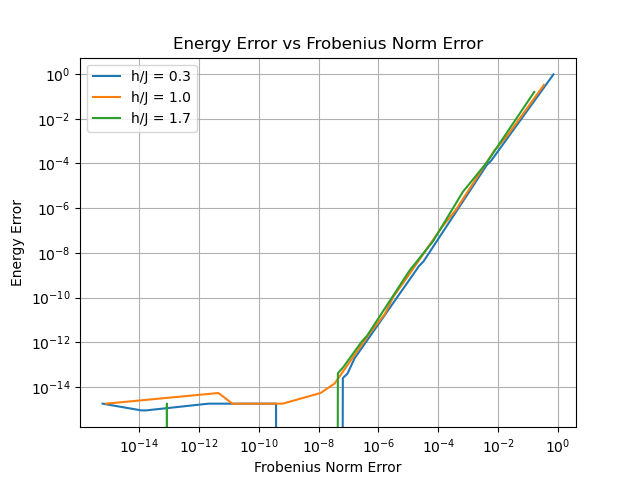
\includegraphics[width=\textwidth]{energy_vs_frobenius_log_log.png}
\caption{Truncation error of the Schmidt decomposition. As can be seen, we see roughly a linear scaling.}
\end{figure}
% Inline Python code in the document
% Inline Python code in the document
\begin{lstlisting}[language=Python]
from hw1 import sparse_hamiltonian
import numpy as np
import matplotlib.pyplot as plt

def schmidt_decomposition(psi, L):
    """Performs Schmidt decomposition at the middle of the chain."""
    cut_psi = psi.reshape(2**(L//2), -1)
    U, s, Vt = np.linalg.svd(cut_psi, full_matrices=False)
    return cut_psi, U, s, Vt

def truncated_state(U, S, Vh, k):
    """Reconstructs the state using only the first k singular values."""
    Sk = np.zeros_like(S)
    Sk[:k] = S[:k]
    flat_psi_k = U @ np.diag(Sk) @ Vh
    return flat_psi_k, flat_psi_k.flatten()

h_values = [0.3, 1, 1.7]
L = 8
errors = {hi: [] for hi in h_values}

# Single loop to handle everything per each h
for hi in h_values:
    # Compute the ground state
    H = sparse_hamiltonian(L, hi, periodic=False)
    eigenvalues, eigenvectors = np.linalg.eigh(H.toarray())
    ground_state = eigenvectors[:, 0]
    
    # Perform Schmidt decomposition
    original, U, s, Vt = schmidt_decomposition(ground_state, L)
    
    # Loop through all possible k values for truncation
    for k in range(1, 2**(L//2) + 1):
        mat_psi_k, flat_psi_k = truncated_state(U, s, Vt, k)
        norm_error = np.linalg.norm(original - mat_psi_k, 'fro')
        psi_k_energy = (flat_psi_k.conj().T @ H @ flat_psi_k) / (flat_psi_k.conj().T @ flat_psi_k)
        energy_error = np.abs(psi_k_energy - eigenvalues[0])
        errors[hi].append((norm_error, energy_error))

# Plotting the results in log-log scale
for hi, error_list in errors.items():
    norm_errors, energy_errors = zip(*error_list)
    plt.plot(norm_errors, energy_errors, label=f'h/J = {hi:.1f}')

plt.xlabel('Frobenius Norm Error')
plt.ylabel('Energy Error')
plt.title('Energy Error vs Frobenius Norm Error')
plt.xscale('log')
plt.yscale('log')
plt.legend()
plt.grid()
plt.savefig('hw2/docs/images/energy_vs_frobenius_log_log.png')

\end{lstlisting}
\newpage

\subsection*{5.4 Entanglement entropy of highly excited states}
Now we will calculate the entanglement entropy $S(\ell; L)$ for an eigenstate in the middle of the many-body spectrum. Here, consider just one value of $h/J$ (e.g., in the paramagnetic phase) and one choice of boundary conditions (e.g., periodic b.c.), but perform a systematic study of $S(\ell, L)$ for several $L$. Note that the sparse eigensolver does not work in the middle of the spectrum, so you will need a full diagonalization and will thus access smaller systems. To avoid complications with resolving degeneracies, consider a few eigenstates corresponding to non-degenerate eigenvalues close to zero energy (which is exactly in the middle of the spectrum in this model). You will see that the entanglement entropy is much larger for states in the middle of the spectrum compared to the band edges and should observe volume law scaling on average.\\
\begin{figure}[h]
\centering
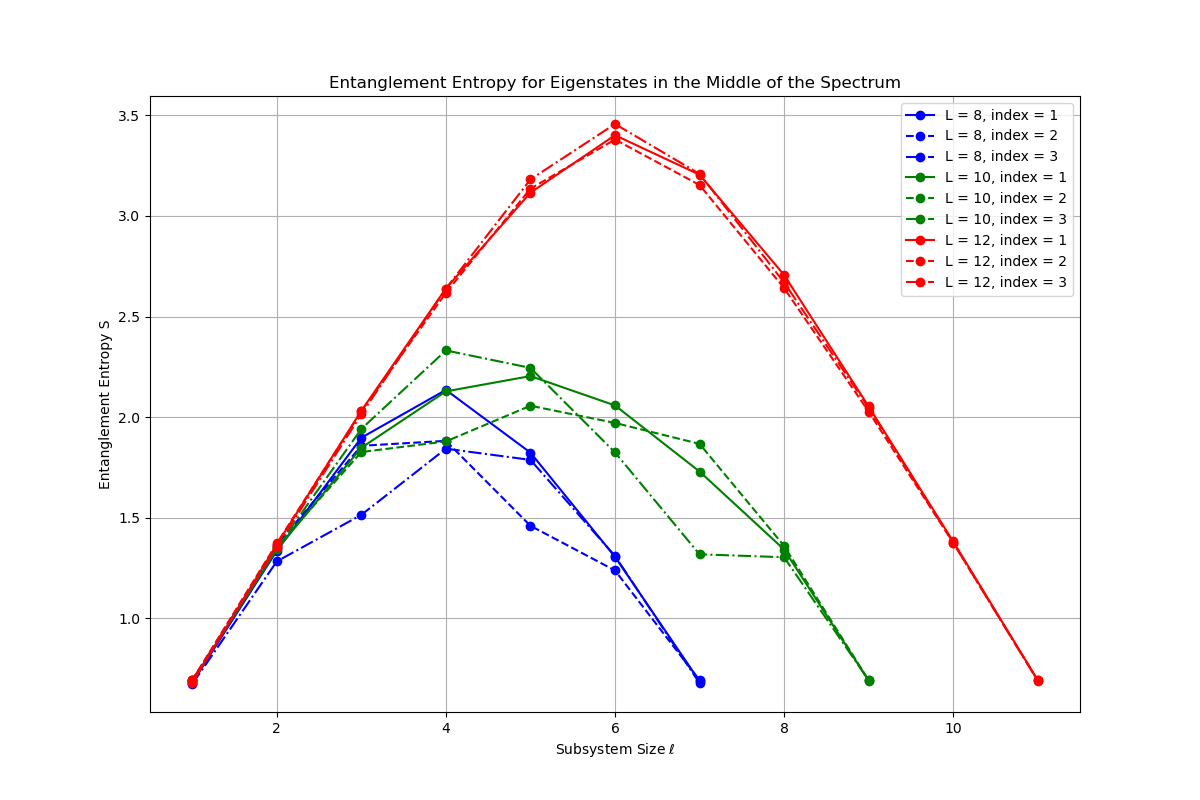
\includegraphics[width=\textwidth]{entanglement_entropy_middle_spectrum.png}
\caption{Entanglement entropy for eigenstates in the middle of the spectrum. I have chosen 3 different states, marked by different indices.}
\end{figure}
What can be observed here is that the entanglement entropy for ground state was close to 0, but in this case, it can range from like 1.0-3.5 for the states in the middle of the spectrum. For the paramagnetic phase that we are considering here, there was 1 ground state to choose from so the entanglement entropy was close to 0. We see a manifestation of the volume law, where the larger system sizes show a larger entanglement entropy. Another observation that can be made is for the smaller system sizes, we were only able to make shorter cuts than for the larger system sizes, so there are fewer data points for this.
% Inline Python code in the document
% Inline Python code in the document
\begin{lstlisting}[language=Python]
from hw1 import periodic_dense_hamiltonian_explicit
from p5_2 import entanglement_entropy, calculate_reduced_density_matrix
import numpy as np
import matplotlib.pyplot as plt

h = 1.7
L_sizes = [8, 10, 12]  # Different system sizes
entropies = {L: {i: [] for i in range(3)} for L in L_sizes}  # Dictionary to store entropies by L and index

for L in L_sizes:
    H = periodic_dense_hamiltonian_explicit(L, h)
    eigenvalues, eigenvectors = np.linalg.eigh(H)

    # Select three eigenstates near the middle of the spectrum
    mid_indices = [len(eigenvalues) // 2 - 1, len(eigenvalues) // 2, len(eigenvalues) // 2 + 1]
    
    for i, mid_index in enumerate(mid_indices):
        state = eigenvectors[:, mid_index]
        
        # Compute the entanglement entropy for each ell using the same procedure as in p5_2.py
        for ell in range(1, L):
            rho_A = calculate_reduced_density_matrix(state, L, ell)
            entropy = entanglement_entropy(rho_A)
            entropies[L][i].append((ell, entropy))  # Store ell and entropy for each index

# Plotting the results
line_styles = ['-', '--', '-.']  # Different line styles for the same system size
colors = ['b', 'g', 'r']  # Different colors for different system sizes

plt.figure(figsize=(12, 8))
for j, L in enumerate(L_sizes):
    for i in range(3):
        ells, L_entropies = zip(*entropies[L][i])  # Unpack ell and entropy values for each L and index
        plt.plot(ells, L_entropies, marker='o', linestyle=line_styles[i], color=colors[j], label=f'L = {L}, index = {i+1}')

plt.xlabel(f'Subsystem Size $\ell$')
plt.ylabel('Entanglement Entropy S')
plt.title('Entanglement Entropy for Eigenstates in the Middle of the Spectrum')
plt.legend()
plt.grid(True)
plt.savefig('hw2/docs/images/entanglement_entropy_middle_spectrum.png')

\end{lstlisting}
\newpage









\end{document}